\documentclass[a0paper,portrait,fleqn,leqno]{tikzposter}
% Ein Blatt in DIN A0 ist 841 mm breit und 1189 mm lang
\title{Wegfindung im Labyrinth}
\institute{Universit\"{a}t Heidelberg}
\author{Florian Nowak \& Yichuan Shen}
%\author{%
%  Florian Nowak\footnote{Florian Nowak: B.\,Sc. Mathematik, 7. Fachsemester}\; \& Yichuan Shen\footnote{Yichuan Shen: M.\,Sc. Mathematik, 1. Fachsemester}\\
%  Betreuer: Gero Plettenberg, Thomas Kloepfer
%  }
\date{Wintersemester 2014/15}

% Für die Bestimmungen aus dem Leitfaden siehe Dokumentende

\settitle{%
  \vspace*{1cm}
  \centering\vbox{%
  \color{titlefgcolor}%
  \hspace{27cm}{\bfseries\Huge\sc\@title}\hspace{8cm}\@titlegraphic\par%
  \vspace*{1em}%
  {\huge\@author\par}
  \vspace*{.75em}
  {\LARGE\@institute\par}%
  \vspace*{.5em}
  {\Large\@date}%
  }}
\tikzposterlatexaffectionproofoff
  
%\settitle{ \centering \vbox{
%\@titlegraphic \\[\TP@titlegraphictotitledistance] \centering
%\color{titlefgcolor} {\bfseries \Huge \sc \@title \par}
%\vspace*{1em}
%{\huge \@author \par} \vspace*{1em} {\LARGE \@institute}
%}}
  
\colorlet{Gray}{black!40}
\colorlet{lightGray}{black!25}
\colorlet{Lime}{lime!50!black!70}
\colorlet{lightLime}{lime!50!black!30}
\colorlet{Blue}{blue!50!black!70}

\definecolorstyle{mystyle}{%
  \definecolor{colorOne}{named}{lightGray}
  \definecolor{colorTwo}{named}{Blue}
  }{%
  % Background Colors
  \colorlet{backgroundcolor}{white}
  \colorlet{framecolor}{colorOne}
  % Title Colors
  \colorlet{titlefgcolor}{black}
  \colorlet{titlebgcolor}{white}
  % Block Colors
  \colorlet{blocktitlebgcolor}{colorTwo}
  \colorlet{blocktitlefgcolor}{white}
  \colorlet{blockbodybgcolor}{white}
  \colorlet{blockbodyfgcolor}{black}
  }
\definelayouttheme{mytheme}{%
  \usecolorstyle{mystyle}
  \usebackgroundstyle{Default} 
  % Predefined Styles: Default, Rays, VerticalGradation, 
  % BottomVerticalGradation, Empty
  \usetitlestyle{Filled} 
  % Default, Basic, Envelope, Wave, VerticalShading, Filled, Empty
  \useblockstyle{Basic}
  % Default, Basic, Minimal, Envelope, Corner, Slide, TornOut
  \useinnerblockstyle{Default} 
  % Default, Table
  \usenotestyle{Sticky} 
  % Default, Corner, VerticalShading, Sticky
  }

\titlegraphic{%
  \includegraphics[width=19cm]{orb}
  % Die Breite des Logos beträgt a + c + c + a = 140,2 mm + 10 mm + 10 mm + 140,2 mm = 300,4 mm für Anwendungen in DIN A0 (siehe Gestaltungshandbuch, Seite 11). Der Abstand des Logos zum oberen sowie zum rechten Rand des Posters beträgt c + d = 10 mm + 20 mm = 30 mm.
  }
\usetheme{mytheme}

\usepackage[ngerman]{babel}
\usepackage{graphicx}
\usepackage[colorlinks=true,urlcolor=cyan,hidelinks]{hyperref}
\usepackage[utf8]{inputenc}
\usepackage[default]{sourcesanspro}

%\usepackage{minted}
%  \usemintedstyle{monokai}
\usepackage{blindtext}


\begin{document}
\maketitle


\begin{columns}
  \column{.5}
  \block[roundedcorners=0,linewidth=2pt]{Aufgabenstellung}{%
  \begin{tikzfigure}%[Roboter mit aufliegendem Labyrinth]
  	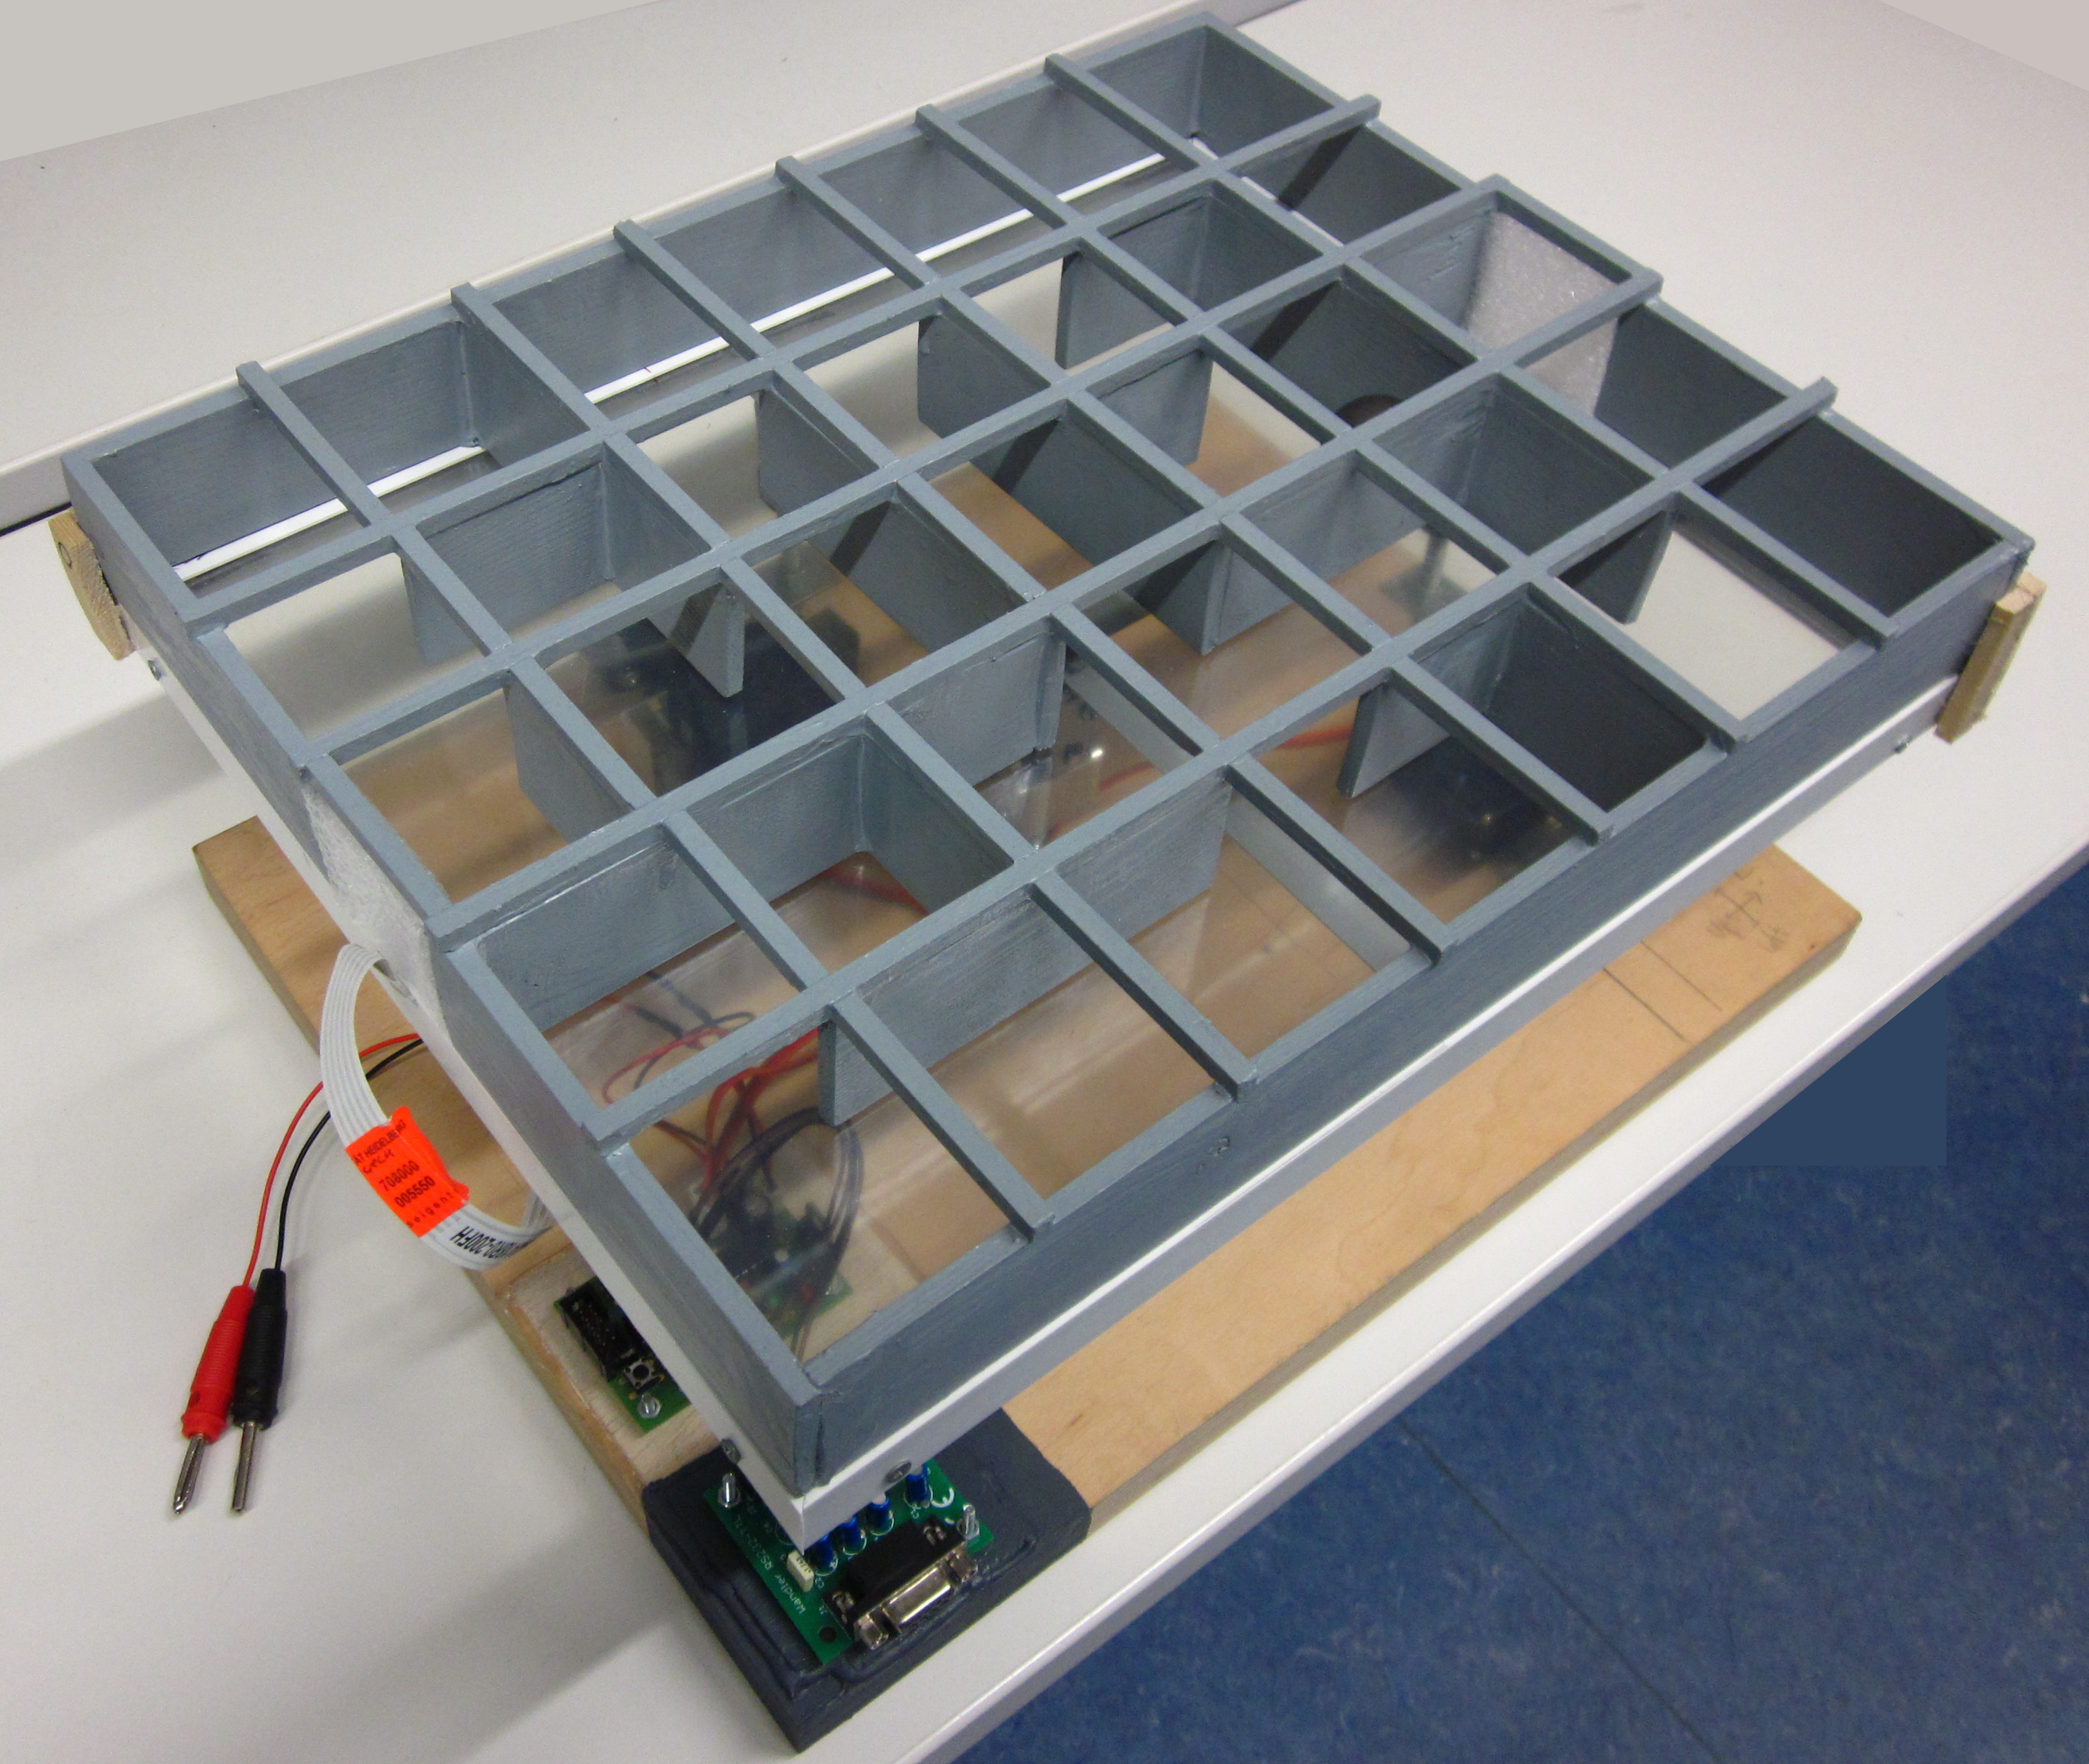
\includegraphics[width=38cm]{roboter_badly-photoshoped}
  \end{tikzfigure}
  \vspace{1em}
  Ein bereits vorhandener Roboter mit neigbarem Touchscreen soll etwas Neues lernen: 
  
  \smallskip\noindent
  Er soll ein beliebiges auf dem Rahmen seines Touchscreens aufliegendes Labyrinth (vorgegebener Rastergröße) mithilfe einer Metallkugel einlesen können. Der Roboter kann eine solche Kugel bereits auf eine ihm vorgegebene Position durch Kippen rollen lassen (und dort auch zum Stillstehen bringen). Das Ziel ist es somit, den Roboter ein zuvor eingelesenes Labyrinth mit der Kugel (auf optimalem Weg) lösen zu lassen.
  }
  \block[roundedcorners=0,linewidth=2pt]{Beteiligte}{%
  %\textbf{Studierende}\\
  \makebox[0pt][l]{\textbf{Florian Nowak:}}\hphantom{Gero Plettenberg}\hspace{1em}B.\,Sc. Mathematik, 7. Fachsemester\\
  \makebox[0pt][l]{\textbf{Yichuan Shen:}}\hphantom{Gero Plettenberg}\hspace{1em}M.\,Sc. Mathematik, 1. Fachsemester
  
  \medskip\noindent
  Gero Plettenberg\hspace{1em}\textit{(Betreuer)}\\
  \makebox[0pt][l]{Thomas Kloepfer}\hphantom{Gero Plettenberg}\hspace{1em}\textit{(Supervisor)} 
  }
  \block[roundedcorners=0,linewidth=2pt]{Sonstiges}{%
  \textbf{GitHub Projektseite:}\hspace{1em}\url{github.com/flo7210/WegfLaby_AP} 
  }
  \column{.5}
  \block[roundedcorners=0,linewidth=2pt]{Überblick}{%
  Text.
  }
  \block[roundedcorners=0,linewidth=2pt]{Labyrintherkennung}{%
  
  }
  \block[roundedcorners=0,linewidth=2pt]{Wanderkennung}{%
  Das folgende Flowchart stellt die (lokale) Wanderkennung dar:
  \vspace{1em} 
  \begin{tikzfigure}
  	\includegraphics[width=38cm]{flowchart_cutout}
  \end{tikzfigure}
  }
  \block[roundedcorners=0,linewidth=2pt]{Lösen des Labirinths}{%
  Wir berechnen den optimalen Pfad durch das Labyrinth per\ldots
  }
\end{columns}

\end{document}

% Auszug aus dem Leitfaden (Abschnitt 7.2):
%
% Das Poster dient dazu, das Ergebnis des Projektes auf eine prägnante und ansprechende Weise darzustellen. Im Gegensatz zur Webpage liegt der Fokus beim Poster auf dem Ergebnis des Praktikums und nicht auf dem Praktikumsverlauf. Das Layout des Posters soll gut strukturiert und optisch ansprechend sein. Zwischen Grafiken und Text soll ein Gleichgewicht herrschen und es soll sichergestellt sein, dass der Betrachter Grafiken dem zugehörigen Text zuordnen kann.
%
% Das Poster beinhaltet folgende Punkte:
% • Titel des Projektes
% • Bearbeitungszeitraum (das jeweilige Semester, in dem das Praktikum absolviert wurde)
% • Name und Studienfächer der Studierenden
% • Betreuer und Supervisor
% • Aufgabenstellung des Projektes
% • Ergebnis
% • Bilder des Roboters, Visualisierung o. Ä.
%
% Das Poster ist in DinA0- oder DinA4- Format als PDF dem jeweiligen Betreuer zu schicken. Auf ausreichende Auflösung der Fotos ist zu achten, außerdem sollten Texte und Graphiken im Vektorformat vorliegen. Die Hintergrundfarbe des Posters ist weiß.